
\section{Global Presentation of the Library}


\texttt{OpenMotion} est une librairie open source qui permet a l'utilisateur d'estimer l'orientation du telephone a partir des donnee de l'IMU. La librairie ne supporte pas encore les translations, nous nous sommes concentre sur l'attitude.



\begin{itemize}
\item The North East Down (NED) frame $\{a\}$ system has its origin fixed at the (moving) object center of gravity. The $z$-axis points upward perpendicularly to the tangent plane of the ellipsoid, and the $x$-axis points towards true north (and not the magnetic north). The $y$-axis point towards east.

\vspace{0.1cm}

\item The object-fixed reference frame $\{c\}$ is a moving and rotating coordinate frame that is fixed to the smartphone device. 
\end{itemize}

The library admit admit that all the components of the IMU belong to the same reference frame $\{c\}$ (ref figure~\ref{Schema_situation}). It is a cyclopean approximation \cite{ouarti2008multimodal} .

\begin{figure}[!h]
\centering
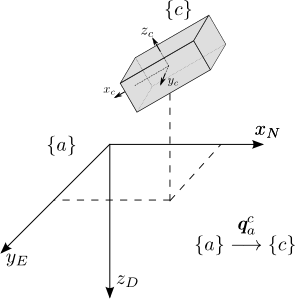
\includegraphics[scale=0.55]{images/Schema_situation.png}
\caption{Definition of the scene with 2 frame:  a fixed frame NED (North East Down) noted $\{a\}$ and a moving frame object noted $\{c\}$}
\label{Schema_situation}
\end{figure}


La librairie donne une estimation le quaternion $\mathbi{q}_a^c$
